% Autor: Simon May
% Datum: 2014-09-17
\section{Die alljährliche Nikolaus-Aktion der Fachschaft Physik}
\begin{multicols}{2}
\textbf{HOHOHO, von draus vom Walde komm ich her\dots\ der Rest ist alt und interessiert keinen mehr.}

{% Fehlermeldungen deaktivieren
\hbadness=10000
% "\columnsep": Verwendet wrapfigure für den Abstand zwischen Text und Bild
\setlength{\columnsep}{0.2cm}
\begin{wrapfigure}{r}[0.4cm]{0cm}
\centering
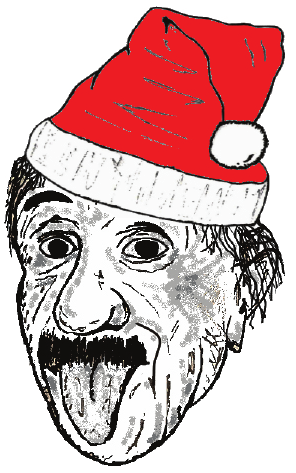
\includegraphics[width=0.55\columnwidth]{res/nikolaus_einstein.png}
\end{wrapfigure}
Jedes Jahr in der Weihnachtszeit habt ihr pünktlich zum 6.\ Dezember die Möglichkeit, euren Kommilitonen eine Freude zu bereiten, denn die Fachschaft~Physik besucht euch in euren Vorlesungen und verteilt Schokoladen-Nikoläuse. Natürlich nicht umsonst, sondern zum Selbstkostenpreis von einem Euro. Diese Aktion gibt es schon seit Jahren und kommt jedes Jahr immer sehr gut beim kompletten Fachbereich an.

Die Aktion wurde ins Leben gerufen, um euch die Chance zu geben, besonderen Menschen einfach mal zu zeigen, dass ihr sie mögt. Egal ob für kopierte Rechenaufgaben, als Motivationshilfe in schwierigen Lebenslagen, oder als Flirtversuch, die Kalorienbomben sind jedes Jahr heiß begehrt und schnell vergriffen. Es wurde sogar schon versucht, Professoren bzgl.\ der schweren Übungszettel/Modulabschlussklausuren zu bestechen, doch wurde bis dato keine signifikante Auswirkung gemessen. Sollte die beschenkte Person nicht in der Vorlesung anwesend sein, kann diese Person den Nikolaus dann noch bis zum letzten Vorlesungstag des laufenden Jahres im Raum der Fachschaft abholen.}

Besucht werden die jeweiligen Pflichtmodule des ersten, dritten und fünften Semesters. Das bedeutet entweder die Mathe- oder Physik-Vorlesungen (je nachdem, welche gerade an dem besagten Tag ist). 2-Fach-Bachelor-Studenten müssen ein wenig aufpassen, wenn die Nikoläuse in den Mathe-Vorlesungen verteilt werden.

Sollte der 6.\ Dezember auf einen Sonn- oder Feiertag fallen, werden die Nikoläuse am folgenden Vorlesungstag von uns ausgeteilt. Die Nikolaus-Aktion wird immer rechtzeitig vorher (auch in euren Vorlesungen) angekündigt, damit ihr die Möglichkeit habt, im Raum der Fachschaft Physik eure Grußkarte zu erwerben. Diese Karte könnt ihr dann kreativ gestalten und uns zurückbringen. Wir kümmern uns dann darum, dass die Karte auch einem Schokoladen-Nikolaus zugeordnet wird und dieser seinen Empfänger auch erreicht.

\fibelsig{Andreas G.}
\end{multicols}

\begin{center}
\includegraphicscompressed[width=0.85\textwidth]{res/nikolaus_foto.png}
\end{center}
